\documentclass[a4paper]{article}
\usepackage[warn]{mathtext}
\usepackage[utf8]{inputenc}
\usepackage[T2A]{fontenc}
\usepackage[english,russian]{babel}
\usepackage{indentfirst}
\usepackage{misccorr}
\usepackage{subcaption}
\captionsetup{compatibility=false}
\usepackage{geometry}
\geometry{verbose,a4paper,tmargin=2cm,bmargin=2cm,lmargin=1.5cm,rmargin=1.5cm}
\usepackage{graphicx}
\usepackage{wrapfig}
\usepackage{amsmath}
\usepackage{fancyhdr}
\usepackage{floatflt}
\usepackage{float}
\usepackage{amssymb}
\usepackage{color}
\usepackage{lscape}
\usepackage{hvfloat}
\usepackage{amsfonts}
\usepackage{euscript}
\usepackage{newunicodechar}
\usepackage{listings}



\usepackage{xcolor}
\usepackage{hyperref}
% Цвета для гиперссылок
\definecolor{linkcolor}{HTML}{000000} % цвет ссылок
\definecolor{urlcolor}{HTML}{000070} % цвет гиперссылок

\definecolor{dkgreen}{rgb}{0,0.6,0}
\definecolor{gray}{rgb}{0.5,0.5,0.5}
\definecolor{mauve}{rgb}{0.58,0,0.82}

\hypersetup{pdfstartview=FitH,  linkcolor=linkcolor,urlcolor=urlcolor, colorlinks=true}

\lstset{
  language=Java,
  aboveskip=3mm,
  belowskip=3mm,
  showstringspaces=false,
  columns=flexible,
  basicstyle={\small\ttfamily},
  numbers=none,
  numberstyle=\tiny\color{gray},
  keywordstyle=\color{blue},
  commentstyle=\color{dkgreen},
  stringstyle=\color{mauve},
  breaklines=false,
  breakatwhitespace=true,
  tabsize=3
}

\begin{document}


\begin{titlepage}
	\centering
    
	\vspace{10cm}
	{\scshape\LARGE  Отчет по практическому заданию №1 \par}
	\vspace{1cm}
	{\huge\bfseries  Объектно-ориентированное программирование в Java\par}
	\vspace{1cm}
	\vfill
\begin{flushright}
	{\large Выполнила:}\par
	\vspace{0.3cm}
	{\LARGE Юлия Прохорова}
\end{flushright}
	
	\vfill

% Bottom of the page
	2021 г.
\end{titlepage}

\newpage

\pagestyle{fancy} 
\fancyhead[R]{ООП в Java}
\fancyhead[L]{Юлия Прохорова}
\fancyhead[C]{}
\fancyfoot{}
\fancyfoot[C]{ \noindent\rule{\textwidth}{0.4pt} \thepage }

\tableofcontents

\newpage

\newcommand{\RNumb}[1]{\uppercase\expandafter{\romannumeral #1\relax}}


\section{\href{https://github.com/julproh/5_sem/tree/main/NetCracker/Java_Basics_and_OOP/first_task/equations}{Решение квадратных уравнений}}

\begin{enumerate}
    \item Реализация программы:
    \begin{lstlisting}
        package equations;

    import java.util.Scanner;

    public class SolvingEquation{ 
        public static void main (String[] args) {
            double[] coefficient = new double[3]; 
            Scanner in = new Scanner(System.in);
            for (int i = 0; i < coefficient.length; i++) {
                coefficient[i] = in.nextDouble(); 
            }
            in.close();
            if (coefficient[0] == 0 && coefficient[1] != 0  ) { 
                System.out.println("Solution: " + -coefficient[2]/coefficient[1] );
            } 
            else if (coefficient[0] == 0 && coefficient[1] == 0 && coefficient[2]!=0) {
                System.out.println("The equation has no solution");
            }
            else if (coefficient[0] == 0 && coefficient[1] == 0 && coefficient[2]==0) {
                System.out.println("The equation has infinitely many solutions");
            }
            else {
                Equations equation_ = new Equations(coefficient[0], coefficient[1], coefficient[2]);
                equation_.answer(equation_.discriminant_.discriminant(equation_.a, equation_.b, equation_.c));
            }
        }
    }

    class Equations {
        public double a, b, c; // a*x*x+b*x+c=0 - equation
        Discriminant discriminant_ = new Discriminant();

        Equations(double a, double b, double c) {
            this.a = a;
            this.b = b;
            this.c = c;
        }

        class Discriminant {
            public double discriminant (double a, double b, double c) {
                double q_discriminant = b*b - 4*a*c;
                double _discriminant;
                if (q_discriminant >= 0) {
                    _discriminant =  Math.sqrt(q_discriminant);
                } 
                else {
                    _discriminant = -1;
                }
                return _discriminant;
            };
        }
    
        public void answer (double _discriminant) {

            if (_discriminant < 0) {
                System.out.println("No Real Solutions");
            }
            else if (_discriminant == 0) {
                System.out.println("Solution: " + -this.b/2/this.a);
            }
            else {
                System.out.println("Solution: " + (-this.b+_discriminant)/2/this.a);
                System.out.println("Solution: " + (-this.b-_discriminant)/2/this.a);
            }
        }
    }

\end{lstlisting}

    \item Результаты тестов:
        
        \begin{figure}[h!]
            \begin{center}
                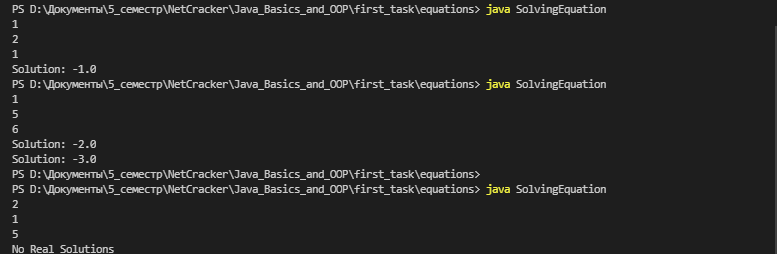
\includegraphics[scale = 0.6]{test_t1.png}
                \label{p2} %% метка рисунка для ссылки на него
            \end{center}
        \end{figure}
    
    \item Структура class файлов:
    
    \item Использование вложенного класса:
    
    

    
\end{enumerate}

\section{\href{https://github.com/julproh/5_sem/tree/main/NetCracker/Java_Basics_and_OOP/first_task/bones}{Игра в кости}} 

    \begin{enumerate}

        \item Реализация программы:
    
        \item Результаты тестов:
    
    \end{enumerate}

\section{\href{https://github.com/julproh}{Адрес человека}}

    \begin{enumerate}
   
        \item Реализация программы:
    
        \item Результаты тестов:
    
    \end{enumerate}

\end{document}